\documentclass[9pt,twocolumn]{article}

\usepackage{amsmath}
\usepackage{graphics}
\usepackage{subfigure}
\usepackage{epsfig}
%\usepackage[margin=0.5in]{geometry}
\usepackage[top=2cm, bottom=2cm, left=2cm, right=2cm]{geometry}
\usepackage{listings}
\usepackage{fontspec}

\usepackage{algorithm}
\usepackage[noend]{algpseudocode}
\usepackage{etoolbox}\AtBeginEnvironment{algorithmic}{\footnotesize}  


\setmainfont[
SizeFeatures = {
  {Size =     -8.41, OpticalSize = 8},
  {Size = 8.41-13.1, OpticalSize = 11},
  {Size = 13.1-20.0, OpticalSize = 19},
  {Size = 20.0-,     OpticalSize = 72}},
Ligatures          = {Required, Common, Contextual, TeX},
Numbers            = {OldStyle, Proportional},
RawFeature         = {expansion  = default},
UprightFeatures    = {RawFeature = {protrusion = mnr}},
BoldFeatures       = {RawFeature = {protrusion = mnrb}},
ItalicFeatures     = {RawFeature = {protrusion = mni}},
BoldItalicFeatures = {RawFeature = {protrusion = mnib}}
]{Minion Pro}
\setsansfont{Calibri}

\newcommand*\Let[2]{\State #1 $\gets$ #2}
\algrenewcommand\alglinenumber[1]{{\sf\footnotesize\addfontfeatures{Colour=888888,Numbers=Monospaced}#1}}
\algrenewcommand\algorithmicrequire{\textbf{Precondition:}}
\algrenewcommand\algorithmicensure{\textbf{Postcondition:}}

\title{\textbf{Impact of dynamic wavelength assignment strategies on interference in WSON}}
\author{Francesco Piccinno}
\date{}

\begin{document}

\maketitle

\section*{Abstract} An effective lightpath routing scheme is proposed, which combines an adaptive routing mechanism \cite{art} with an interference aware frequency band allocation. The proposed solution is able to outperform classic RWA schemes and it allows a much greater quality in optical traffic transmission with the least blocking probability as possible.


\section{Introduction}

Wavelength Switched Optical Networks (in short WSON) have been attracting considerable interest in the recent years. This interest is demonstrated by the great number of research projects carried out by academia and industry. This short technical paper tries to offer a new perspective in the direction of a new series of dynamic wavelength assignment strategies that account for new metrics such as low average interference level.

The final goal of this work is to present a novel yet simple modification to a classical routing algorithm jointly with a simple slot allocation heuristic, which allows an outstanding performance measured in terms of blocking probability and average interference level.

The conclusions are mainly derived by a centralized simulation study focused on a real topology, namely the European Optical Network (EON) topology depicted in Figure \ref{fig:topology}. The EON is a transparent all-optical network which interconnects major centers in Europe via high capacity pipes. It is a mesh network composed by a relatively small number of nodes interconnected by links which span several kilometers. In order to provide a worst-case estimate of our solution we treated every single node as a transparent node not capable of carrying out any wavelength conversion.

In this case a given lightpath is subjected to wavelength continuity constraint. The constraint can be expressed as follows: having wavelength $w_1$ been chosen as carrier for a given lightpath, the wavelength $w_1$ must be allocated on every link that are part of the computed lightpath.

\begin{figure}[!htb]
	\centering
	\includegraphics[width=0.4\textwidth]{topology.pdf}
	\caption{European Optical Network Topology}
	\label{fig:topology}
\end{figure}

It is worth pointing out that the proposed solution is essentially a centralized solution with source routing based on a link-state approach. Therefore the scheme can be only adopted on a WSON which adopts a link-state routing strategy, such as OSPF routing or a network employing a centralized Path Computation Element (PCE).

\section{Routing and slot assignment}

As already pointed out, a transparent WSON is considered with $E$ nodes and $V$ bi-directional links. Each of the link supports $N$ slots of bandwidth $B$. Given a pair $(S, D)$ where $S,D \in V$ and $S \ne D$, the routing problem consists in finding a path $(V_1, V_2, \cdots, V_n)$ connecting $S$ to $D$. In case of a network with no wavelength converters, slot assignment problem consists in finding a slot $N_x$ common to all the links, that can be allocated on the entire path returned by solving the routing problem. 

Several algorithms exist that solve these problems by trying to minimize a given metric. The most known algorithm for solving the routing problem, is \emph{Dijkstra's shortest path algorithm}, whose aim is to minimize the cost of the resulting path. On the other hand, \emph{FirstFit} is the simplest and most used heuristic for solving slot assignment problem, and its goal is to minimize the blocking probability.

Since the focus of this work is to propose a solution that offer the lowest average interference level as possible, while not impacting on other metrics, it is useful at this point to introduce Equation \ref{eq:interf}. The formula can be used to derive the interference level perceived by a given slot $x$ ($x \in S$) on a link $L$ (providing $S$ slots).

% interference(x, S_{active}) =
\begin{equation}
\label{eq:interf}
\sum_{i=0}^{S_{active}}\log\left(\frac{\left(|x-i|\times2\right)+1}{\left(\left(|x-i|-1\right)\times2\right)+1}\right)
\end{equation}

In order to better understand the problem and successively design proper heuristics, Equation \ref{eq:interf} was used to derive the plots reported in Figure \ref{fig:gen-diff}. The first figure summarizes the difference in interference level between the \emph{Center} and \emph{Side} allocation on a link offering $32$ slots. The \emph{Center allocation} curve was obtained by fixing as the \emph{target slot} the $16$-th slot. At each iteration, one free slot from the right (in case of even iteration number) or from the left (in case of odd iteration number) is gradually allocated until bandwidth saturation. Similarly, the \emph{Side allocation} curve was obtained by fixing the $32$-th slot as a target slot, while gradually allocating new slots from the right ($1, 2, \ldots, 31$-th).

The second figure presents an histogram realized by taking in consideration a link with $20$ available slots and analyzing all the possible combinations ($2^{20}$). The $x$ axis represents the optimal slot that minimize the interference level, while the $y$ axis represents the number of times a given slot position was selected.

\begin{figure}[!htb]
	\subfigure[Central allocation and side allocation]{
		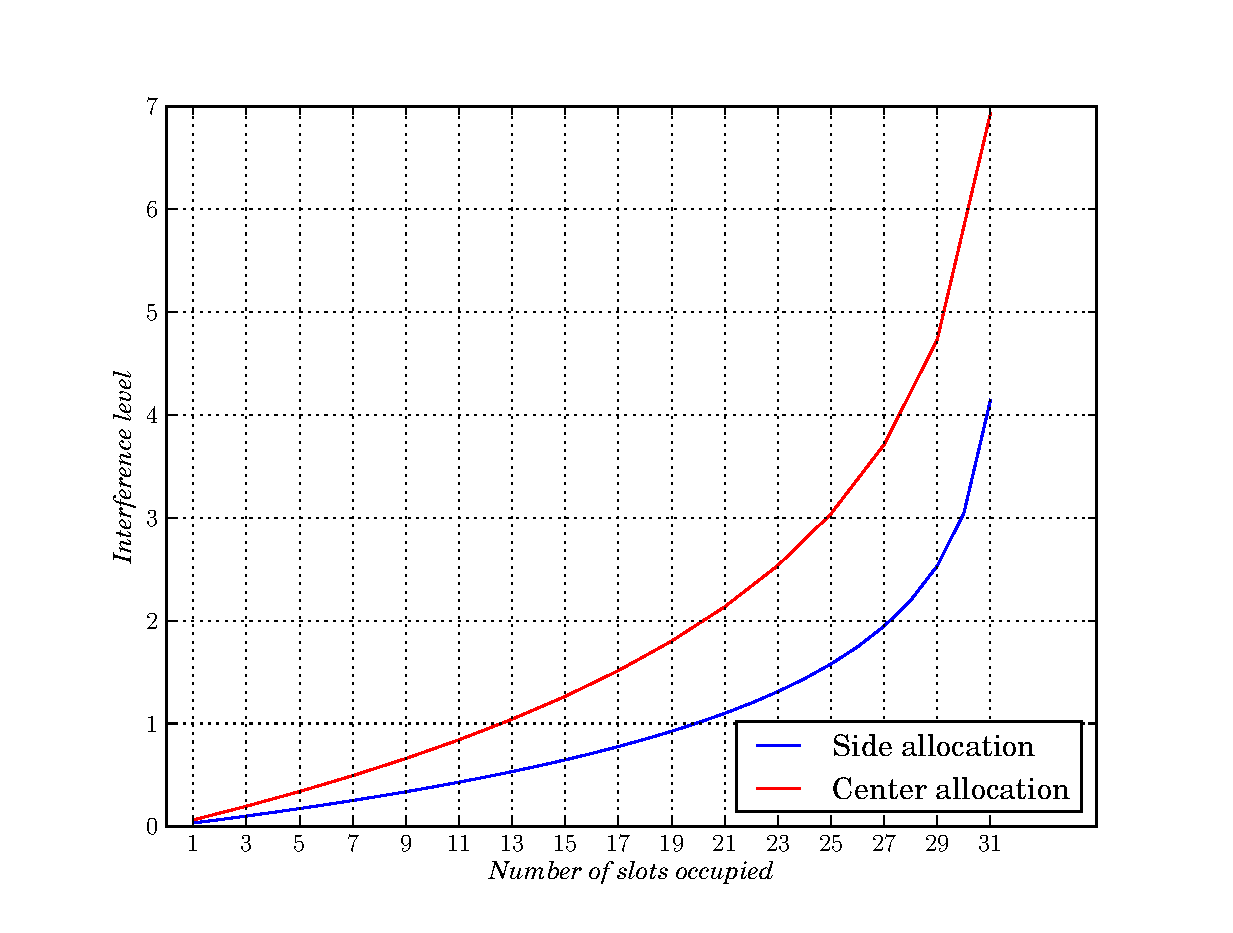
\includegraphics[width=0.45\textwidth]{generic.eps}
		\label{fig:diff}
	}
	\subfigure[Average interference]{
		\includegraphics[width=0.45\textwidth]{precompute.eps}
		\label{fig:histo}
	}
	\label{fig:gen-diff}
	\caption{General considerations about interference}
\end{figure}

By analyzing the two figures, you can easily realize that the winning strategy for achieving the minimum interference level is side allocation. Moreover, an interesting fact emerging from Figure \ref{fig:histo} is that in general is better to avoid the allocation of the second and the second-last slot whenever possible, at least probabilistically speaking.

With this idea in mind, a simple variation of Dijkstra shortest path algorithm was evaluated (Algorithm \ref{alg:sp}). During its operation the procedure tries to keep in consideration both the distance and the available slots. The objective of the procedure is to select the shortest path in terms of distance which has the greater number of available slots, in order to have more space to introduce optimization. This result is then used in the slot assignment procedure (Algorithm \ref{alg:alloc}).

Regarding slot assignment strategies, four different heuristics were analyzed:

\begin{description}
	\setlength{\itemsep}{1.5pt}
	\setlength{\parskip}{0pt}
	\setlength{\parsep}{0pt}

	\item[First Fit] In this schema the first available slot, starting from the left, is allocated.

	\item[First Fit / Last Fit] This heuristic allocates the first available slot that is located as farther as possible from the center.

	\item[First Fit / Last Fit 2] This heuristic is the same as FFLF with the only difference that it prefers to skip the allocation of the second and second-last slot, if possible. The choice is justified by the histogram shown in Figure \ref{fig:histo}.

	\item[MinCost] This method allocates the slot that has the minimum cost among all the possible available slots. This method provides a lower bound for the interference level.
\end{description}

\section{Implementation and Results}

The performance of the proposed algorithm was evaluated by using a custom Python event-driven simulator. \emph{Lightpath setup requests}, represented as a tuple $(S, D)$, are generated by a Poisson process that is exponentially distributed with parameter $\lambda$. Upon reception of a request, the PCE is in charge of allocating a given slot $N_x$, possibly on the shortest path connecting $S$ to $D$. If the lightpath allocation is successful, the simulator generates a \emph{tear-down request} event with exponential distribution of parameter $\mu$. A blocking situation occurs in case the setup request cannot be handled, that is all the slots on the given path are already occupied by other lightpath requests.

As you can see, the simulator is acting as a centralized PCE, which has all the needed link-state information representing the network state at a given time. The PCE is responsible of maintaining the traffic engineering database with detailed and updated slot availability information.

The results of our simulation are presented in Figure \ref{fig:results1} and Figure \ref{fig:results2}. All the points of the graphs were evaluated with a confidence level of 95\%, except for the last two graphs were no confidence interval was considered. The curves were obtained keeping the value of $\mu$ fixed to $1$ while varying the value of $\lambda$ in the interval $80$ - $150$. We analyzed five different strategies:

\begin{itemize}
	\setlength{\itemsep}{1pt}
	\setlength{\parskip}{0pt}
	\setlength{\parsep}{0pt}
	\item Classic routing - First Fit
	\item Adaptive routing - First Fit
	\item Adaptive routing - First Fit / Last Fit
	\item Adaptive routing - First Fit / Last Fit - Skip 2
	\item Adaptive routing - MinCost
\end{itemize}

\begin{figure}[!htb]
	\subfigure[Average Interference Level impact]{
		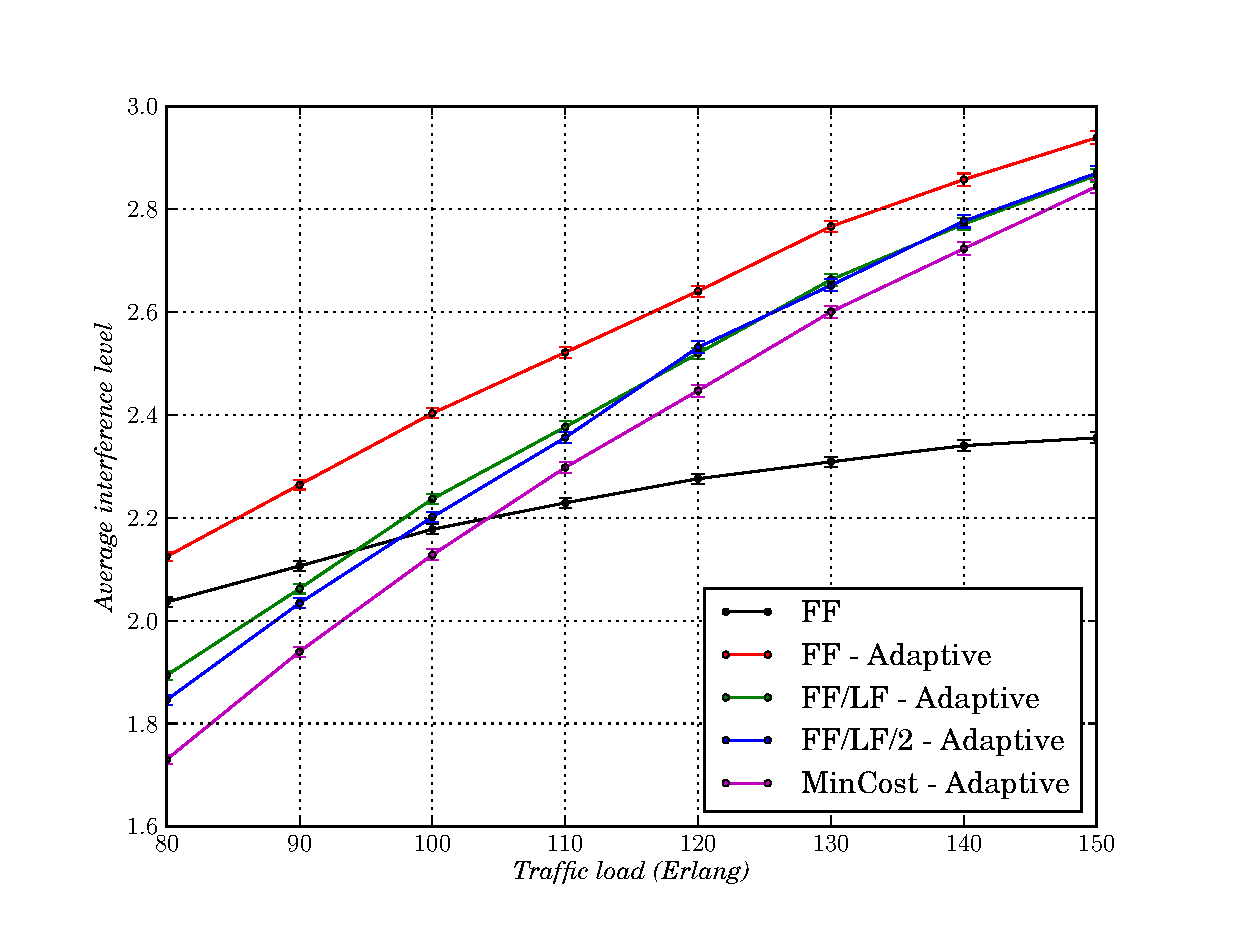
\includegraphics[width=0.49\textwidth]{interference.eps}
		\label{fig:graph}
	}
	\subfigure[Blocking Probability impact]{
		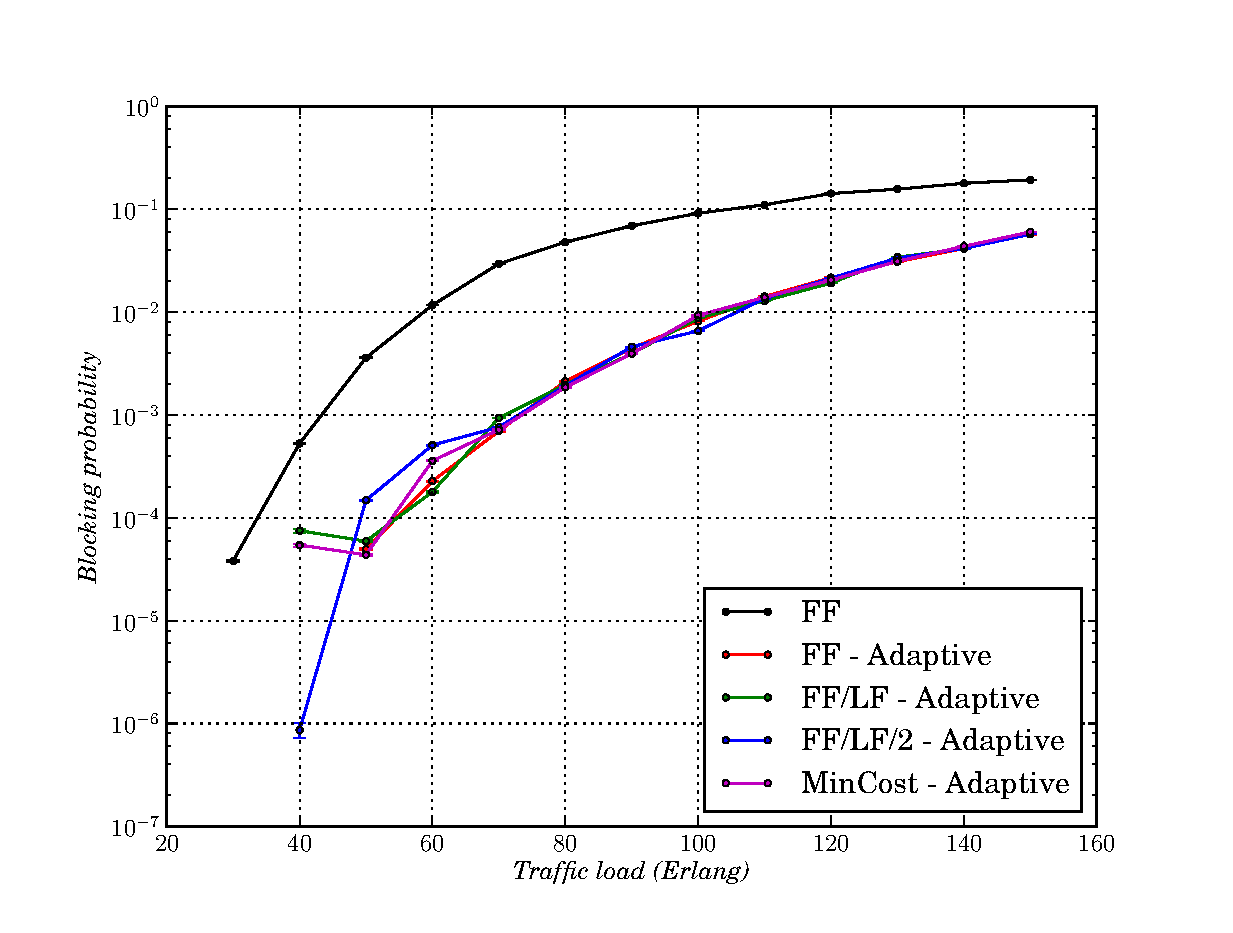
\includegraphics[width=0.49\textwidth]{blocking.eps}
		\label{fig:graph-block}
	}
	\label{fig:results1}
	\caption{Average Interference and Blocking Probability}
\end{figure}

\begin{figure}[!htb]
	\subfigure[Pdf relative to the number of hops]{
		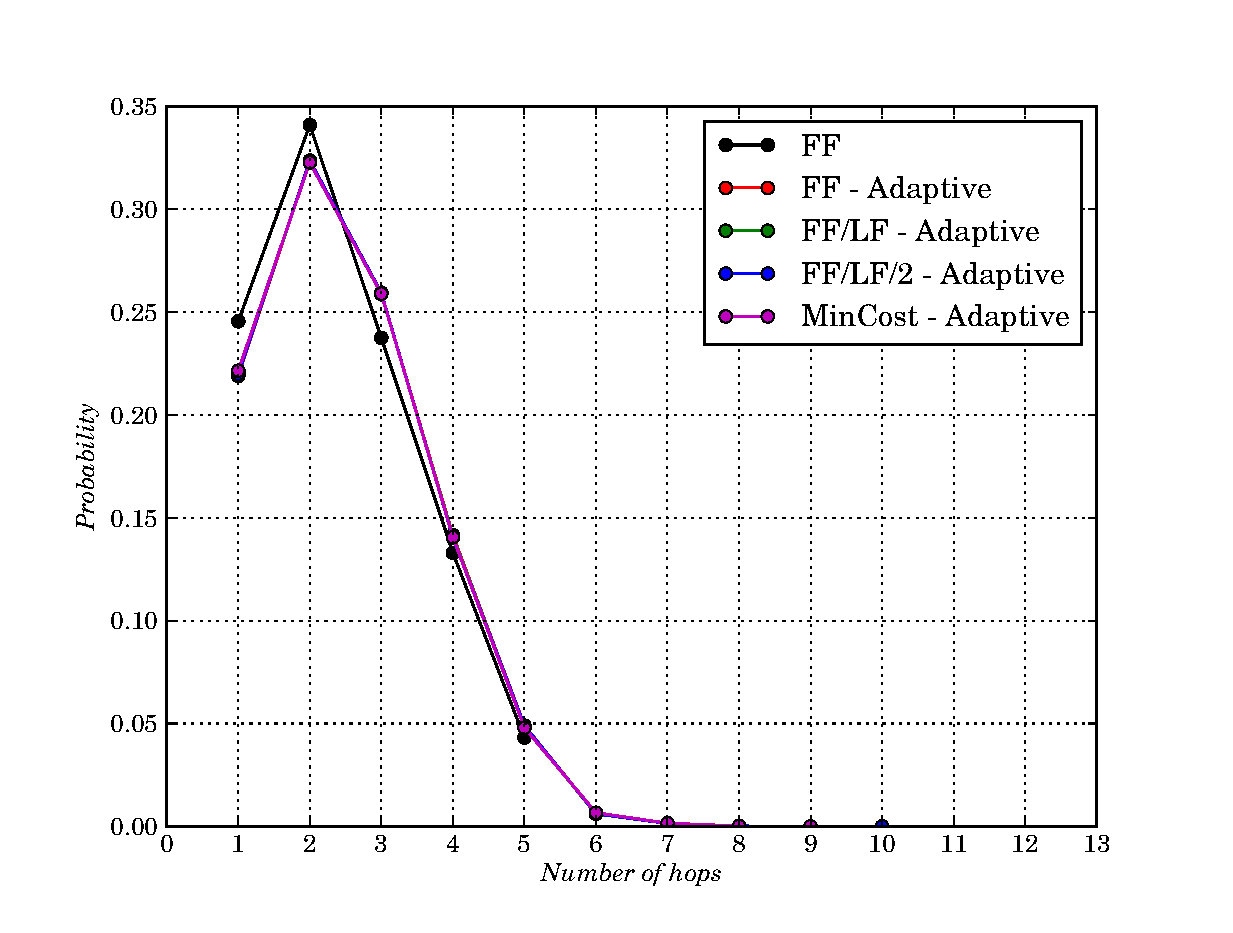
\includegraphics[width=0.49\textwidth]{distance.eps}
		\label{fig:graph-distance}
	}
	\subfigure[Average interference level in function of the number of hops]{
		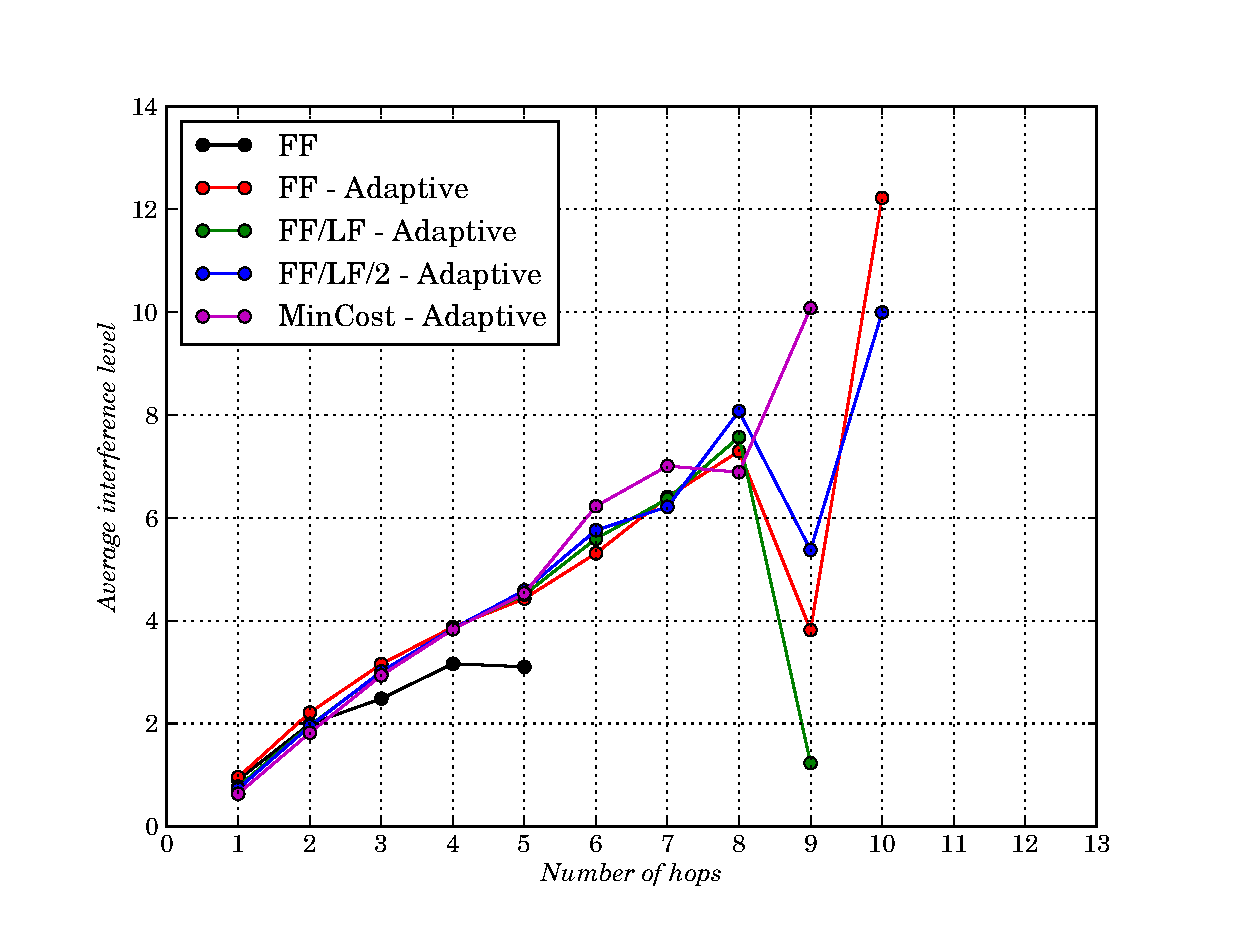
\includegraphics[width=0.49\textwidth]{pdf.eps}
		\label{fig:graph-avg}
	}
	\label{fig:results2}
	\caption{Averaged metrics (80-150 Erlang)}
\end{figure}


Figure \ref{fig:graph} shows the Average Interference Level in function of the Traffic Load. By just taking in consideration the adaptive solutions you can see that FF is the worse, while the MinCost constitutes the theoretical lower bound for this metric. Both FFLF and FFLF2 performs almost the same, with a slight advantage on lower load for the latter. In general all the adaptive solutions converges at higher load. The subtle thing to point out in this graph is that although the classic FF solution seems to be best, it is actually the worst solution possible. Indeed it has a lower interference level curve but this result is paid back by an higher blocking probability.

To this end you can take a look at Figure \ref{fig:graph-block}, which summarizes the blocking probabilities of the various solutions on a larger load range. The plot clearly shows the difference between the adaptive and the classic routing approach and suggests a convergence condition in case of high load traffic conditions. For low load the interpretation is more difficult to draw general conclusions since the results are mainly dependent on the initial random seed and from the network topology.

The conclusions are similar also regarding the PDF graph relative to the number of hops, which is shown in Figure \ref{fig:graph-distance}. As you can see, the classic routing experiences a an abnormal interruption at hop number 5, due to traffic saturation and the relative impossibility of serving any further lightpath setup request.

The last graph, Figure \ref{fig:graph-avg}, shows the behavior of the strategies in function of the number of hops and interference levels. The more you look outside the 0-4 hops interval the less precise is the observation. This is confirmed also by the PDF of the distance previously discussed. As you can see the algorithms presented perform almost the same on this interval. Out of it any conclusion is just speculation, since also the number of samples per point decreases quickly. To draw some kind of conclusion a more long simulation with a very large number of iterations is needed.

\onecolumn
\begin{algorithm}[!h]
	\caption{Slot aware Dijkstra's shortest path algorithm
		\label{alg:sp}
	}
	\begin{algorithmic}[1]
	\Require{$G$ is the graph while $S$ and $D$ are vertexes.}
	\Statex
	\Function{ShortestPath}{$G, S, D$}
		\Let{$Distances$}{\textsc{Hash()}}
		\Let{$Paths$}{\textsc{Hash()}}
		\Let{$Seen$}{\textsc{Hash()}}
		\Let{$Queue$}{\textsc{Queue()}}

		\State $Paths$.set($S$, \textsc{List($S$)})
		\State $Seen$.set($S$, $0$)

		\If{S = D}\State \Return{$\left<0, 0, paths\right>$} \EndIf

		\State $Queue$.\textsc{enqueue($\left<0, S, 0\right>$)}

		\While{ \textbf{not} $Queue$.\textsc{IsEmpty()}}
			\Let{$\left<V_{distance}, V, V_{bandmask}\right>$}{$Queue$.\textsc{ExtractMin()}}
			\If{$Distances$.\textsc{Contains($V$)}} \State \textbf{continue} \EndIf
			\State $Distances$.\textsc{Set($V$, $V_{distance}$)}

			\If{$V = D$} \State \textbf{break} \EndIf
			
			\For{$\left<X, E_{vx}\right> \gets V.$\textsc{AdjacencyList}}
				\Comment{$E_{vx}$ is the edge object connecting $V$ to $X$}
				\State $distance_{vx} \gets Distances$.\textsc{Get}($V$) + $E_{vx}$.\textsc{GetDistance()}
				\State $bandmask_{vx} \gets E_{vx}.$\textsc{GetBandMask()}
				\State $slots_{occupied} \gets $\textsc{GetActiveBits($bandmask$)}

				\State $band \gets bandmask_{vx} \oplus V_{bandmask}$
				\Comment{$\oplus$ is the bitmask OR operation}

				\If{ $\overline{band} \ne 0 $ \textbf{and not} $Seen.$\textsc{Contains($X$)}}
					\State $Seen.$\textsc{Set($X$, $distance_{vx}$)}
					\State $Queue.$\textsc{Enqueue($\left< distance_{vx}, slots_{occupied}, V, band \right>$)}
					\Let{$path_{vx}$}{$Paths.$\textsc{Get($V$)}}
					\State{$path_{vx}.$\textsc{Append(X)}}
					\State $Paths.$\textsc{Set($X$, $path_{vx}$)}
				\EndIf
			\EndFor
		\EndWhile

		\State \Return{$\left<Distances, Paths\right>$}

	\EndFunction
	\end{algorithmic}
\end{algorithm}

\begin{algorithm}[!h]
	\caption{Interference aware allocation strategy
		\label{alg:alloc}
	}
	\begin{algorithmic}[1]
	\Require{$G$ is the graph while $S$ and $D$ are respectively source and destination vertexes.}
	\Statex
	\Function{SlotAssign}{$G, S, D$}
		\Let{$ \left< Distances, Paths \right> $}{\textsc{ShortestPath($G$, $S$, $D$)}}
		\Let{$Path$}{$Paths.$\textsc{Get($D$)}}
		\Let{$Distance$}{$Distances.$\textsc{Get($D$)}}
		\Let{$BitMask$}{$0$}
		\For{$Link \in Path$}
			\Let{$BitMask$}{$BitMask \oplus Link.$\textsc{GetBandMask()}}
		\EndFor
		\Let{$Position$}{\textsc{Allocate($BitMask$)}}
		\Comment{Invoke FirstFit, FirstFitLastFit, FirstFitLastFitSkip2 or MinCost}
		\For{$Link \in Path$}
			\State{$Link.$\textsc{Allocate($Position$)}}
		\EndFor
	\EndFunction

	\Function{FirstFit}{$BitMask$}
		\State \Return{the first free bit in $BitMask$}
	\EndFunction

	\Function{FirstFitLastFit}{$BitMask$}
		\State \Return{the first free bit, either from the left or from the right, of $BitMask$}
	\EndFunction

	\Function{FirstFitLastFitSkip2}{$BitMask$}
		\State \Return{the first free bit, either from the left or from the right, of $BitMask$ avoiding second slot if possible}
	\EndFunction

	\Function{MinCost}{$BitMask$}
		\State \Return{the free bit with least possible interference cost}
	\EndFunction
	\end{algorithmic}
\end{algorithm}

\bibliographystyle{IEEE}
\bibliography{bibliography}
\end{document}
